

\begin{frame}{History of OpenCL}

\begin{minipage}{0.6\textwidth}
\begin{block}{Prior to 2008}
  \begin{itemize}
   \item OpenCL developed by Apple Inc.
  \end{itemize}
\end{block}
\end{minipage} \hfill
\begin{minipage}{0.2\textwidth}
 
\includegraphics[width=0.99\textwidth]{figs/opencl.jpg}
\end{minipage}


\begin{block}{2008}
  \begin{itemize}
   \item OpenCL working group formed at Khronos Group
   \item OpenCL specification 1.0 released
  \end{itemize}
\end{block}

\begin{block}{2010}
  \begin{itemize}
   \item OpenCL 1.1 (multi-device, subbuffer manipulation)
  \end{itemize}
\end{block}

\begin{block}{2011}
  \begin{itemize}
   \item OpenCL 1.2 (device partitioning)
  \end{itemize}
\end{block}

\end{frame}

%%%%%%%%%%%%%%%%%%%%%%% Device %%%%%%%%%%%%%%%%%%%%%%


% \begin{frame}{OpenCL Platform Model}
%  \begin{center}
%    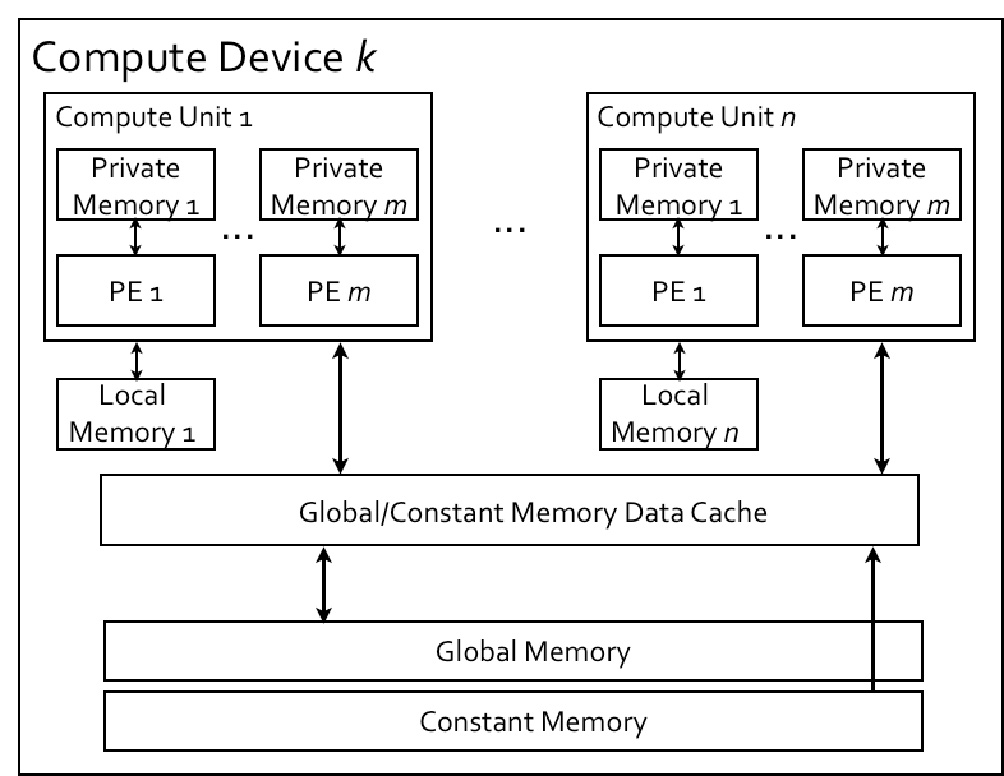
\includegraphics[width=0.8\textwidth]{figs/opencl-device.jpg} \\
%  \end{center}
%   {\tiny http://developer.amd.com/documentation/articles/PublishingImages/opencl\_figure5.jpg}
%   \vspace{0.5cm}
% \end{frame}


%%%%%%%%%%%%%%%%%%%% Platform Model %%%%%%%%%%%%%%%%%%%%%%

\begin{frame}{OpenCL Platform Model}
 \begin{center}
   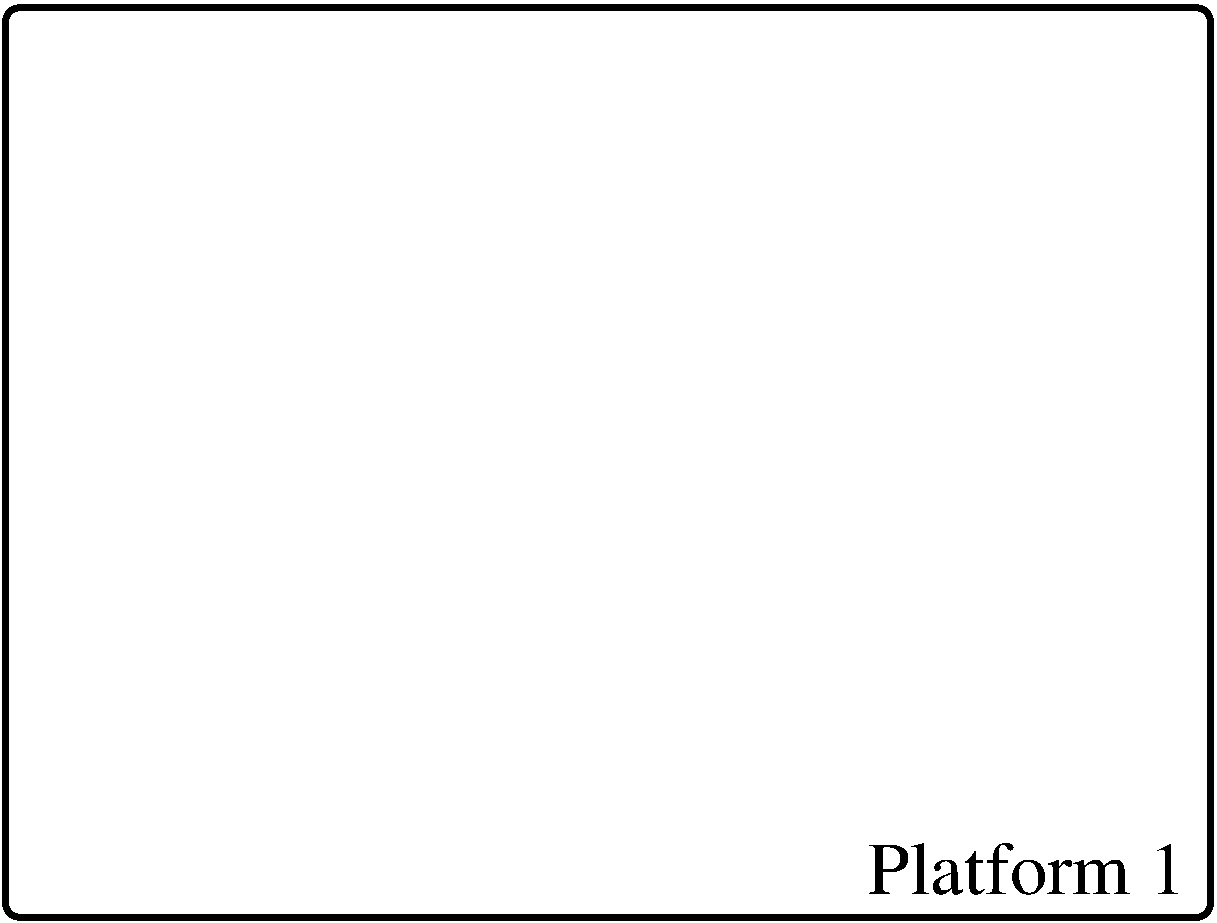
\includegraphics[width=0.85\textwidth]{figs/opencl-2.pdf}
 \end{center}
\end{frame}

\begin{frame}{OpenCL Platform Model}
 \begin{center}
   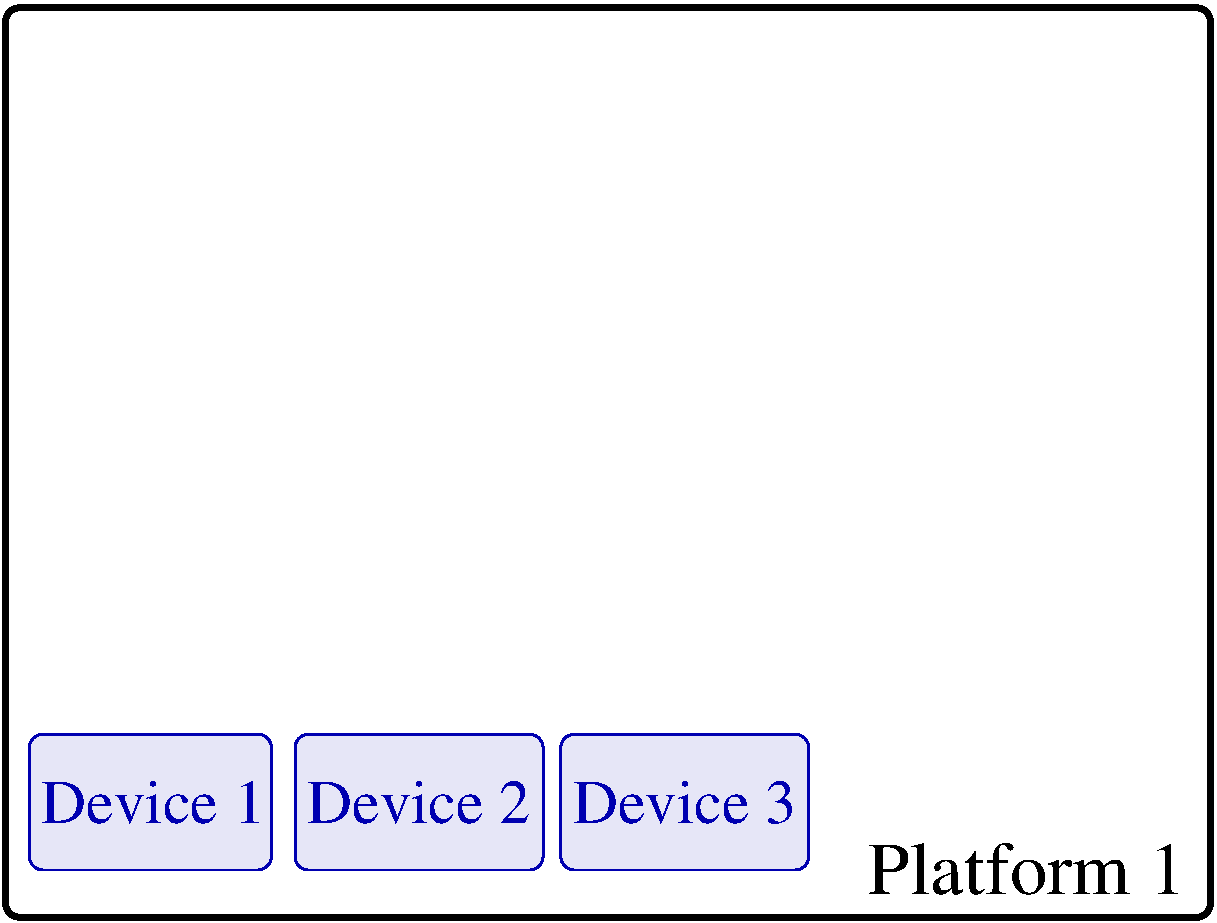
\includegraphics[width=0.85\textwidth]{figs/opencl-3.pdf}
 \end{center}
\end{frame}

\begin{frame}{OpenCL Platform Model}
 \begin{center}
   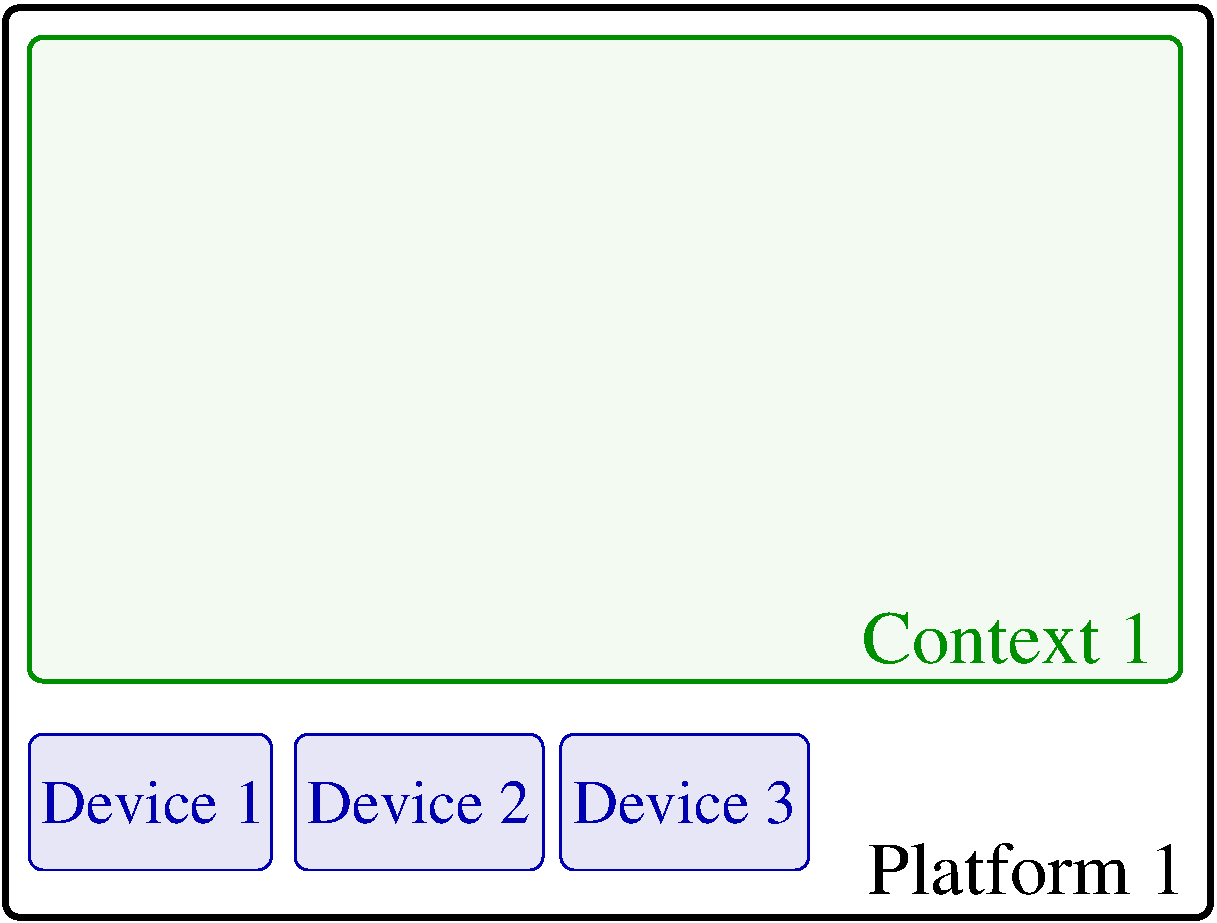
\includegraphics[width=0.85\textwidth]{figs/opencl-4.pdf}
 \end{center}
\end{frame}

\begin{frame}{OpenCL Platform Model}
 \begin{center}
   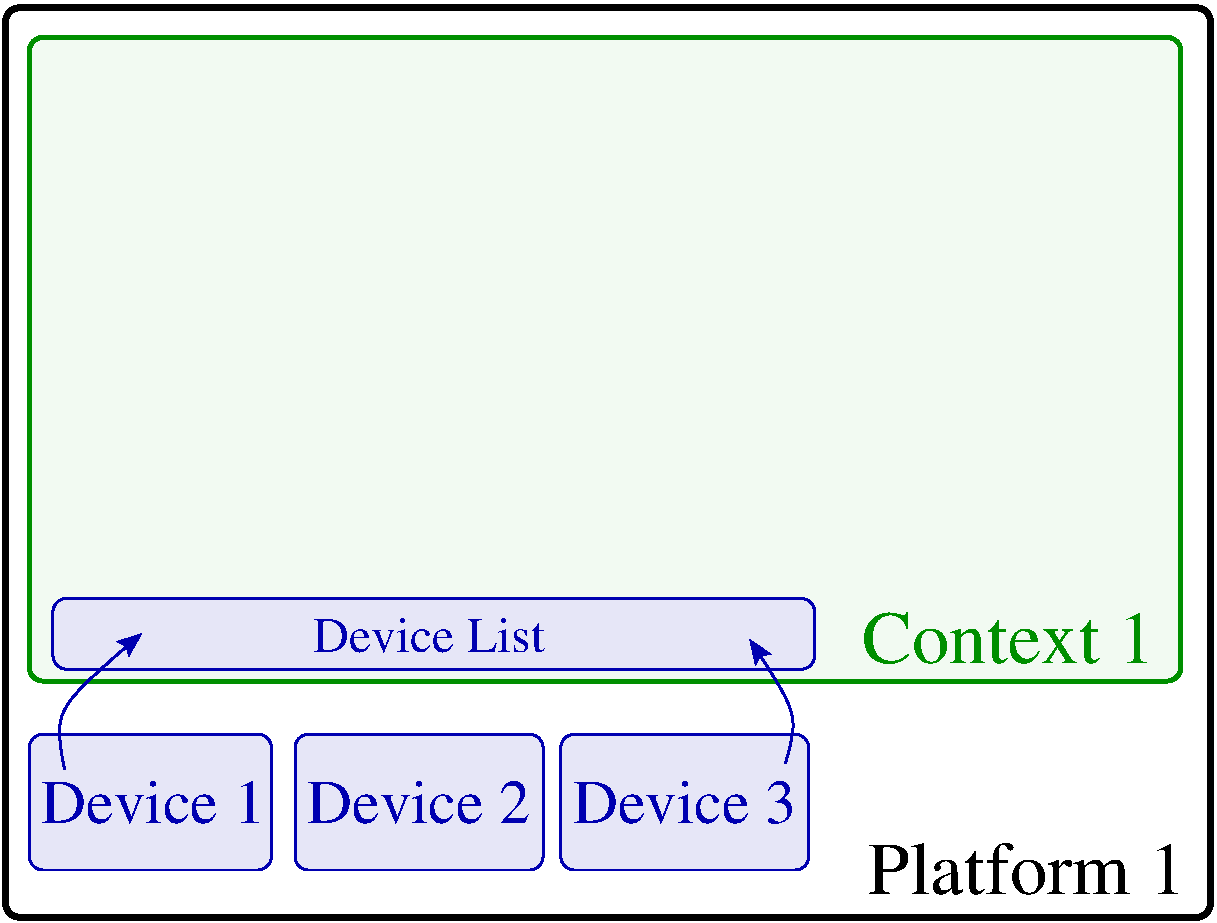
\includegraphics[width=0.85\textwidth]{figs/opencl-5.pdf}
 \end{center}
\end{frame}

\begin{frame}{OpenCL Platform Model}
 \begin{center}
   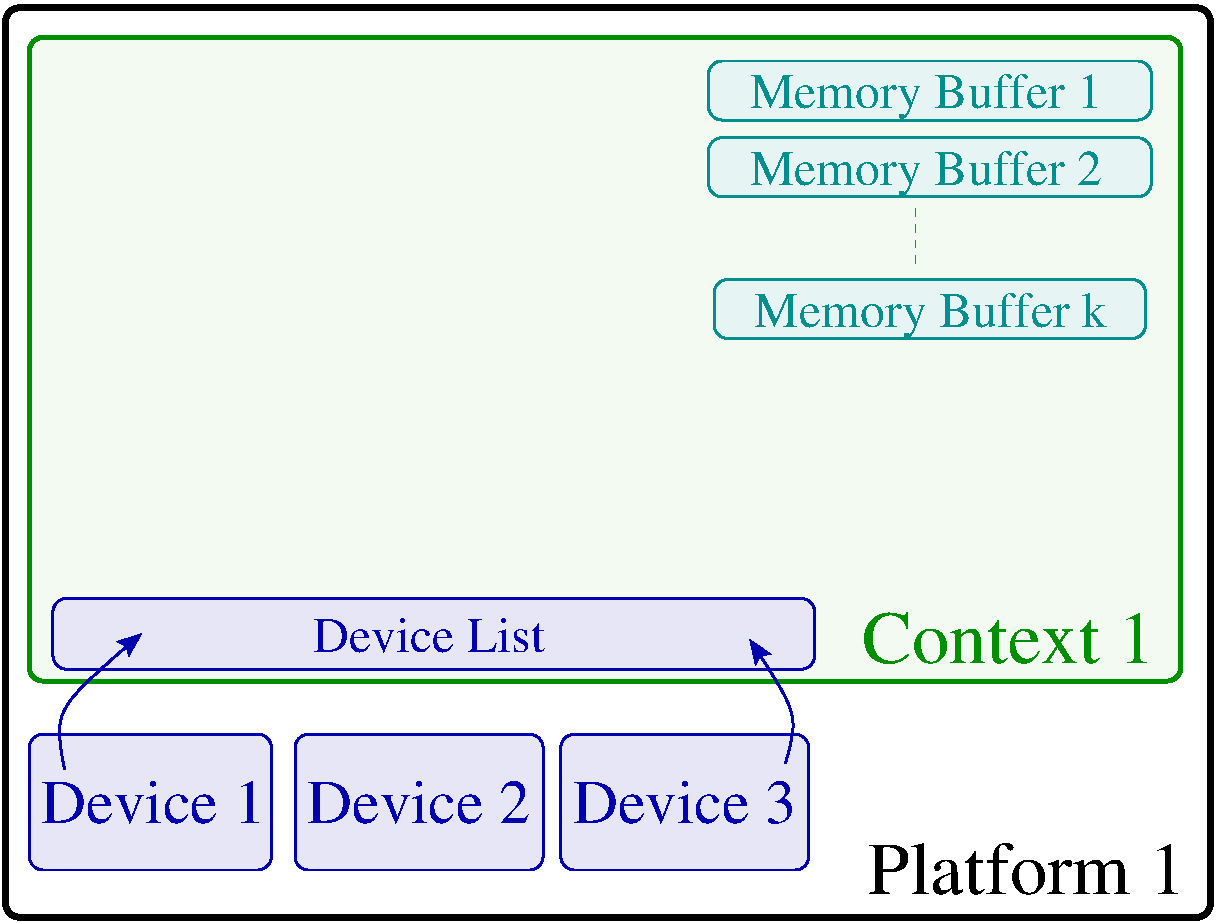
\includegraphics[width=0.85\textwidth]{figs/opencl-6.pdf}
 \end{center}
\end{frame}

\begin{frame}{OpenCL Platform Model}
 \begin{center}
   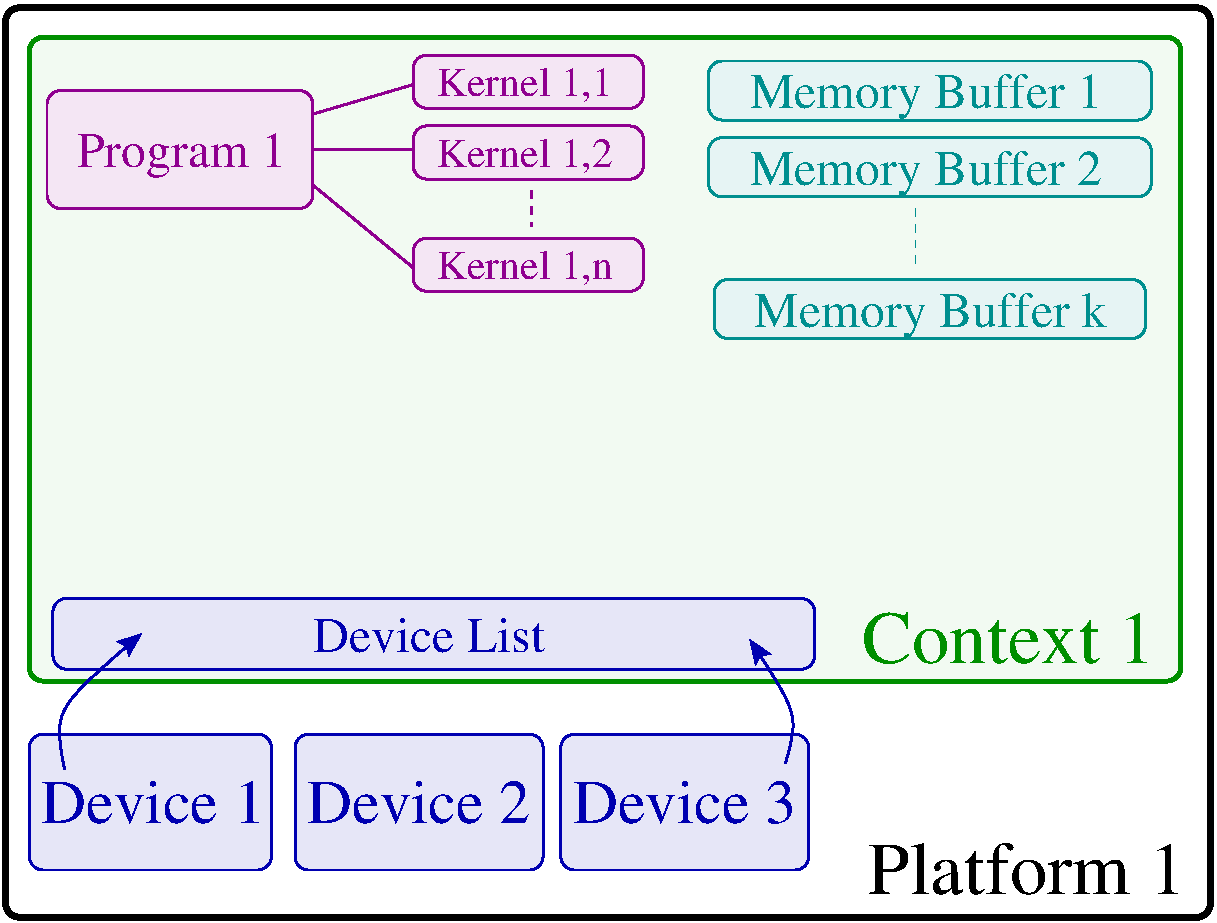
\includegraphics[width=0.85\textwidth]{figs/opencl-7.pdf}
 \end{center}
\end{frame}

\begin{frame}{OpenCL Platform Model}
 \begin{center}
   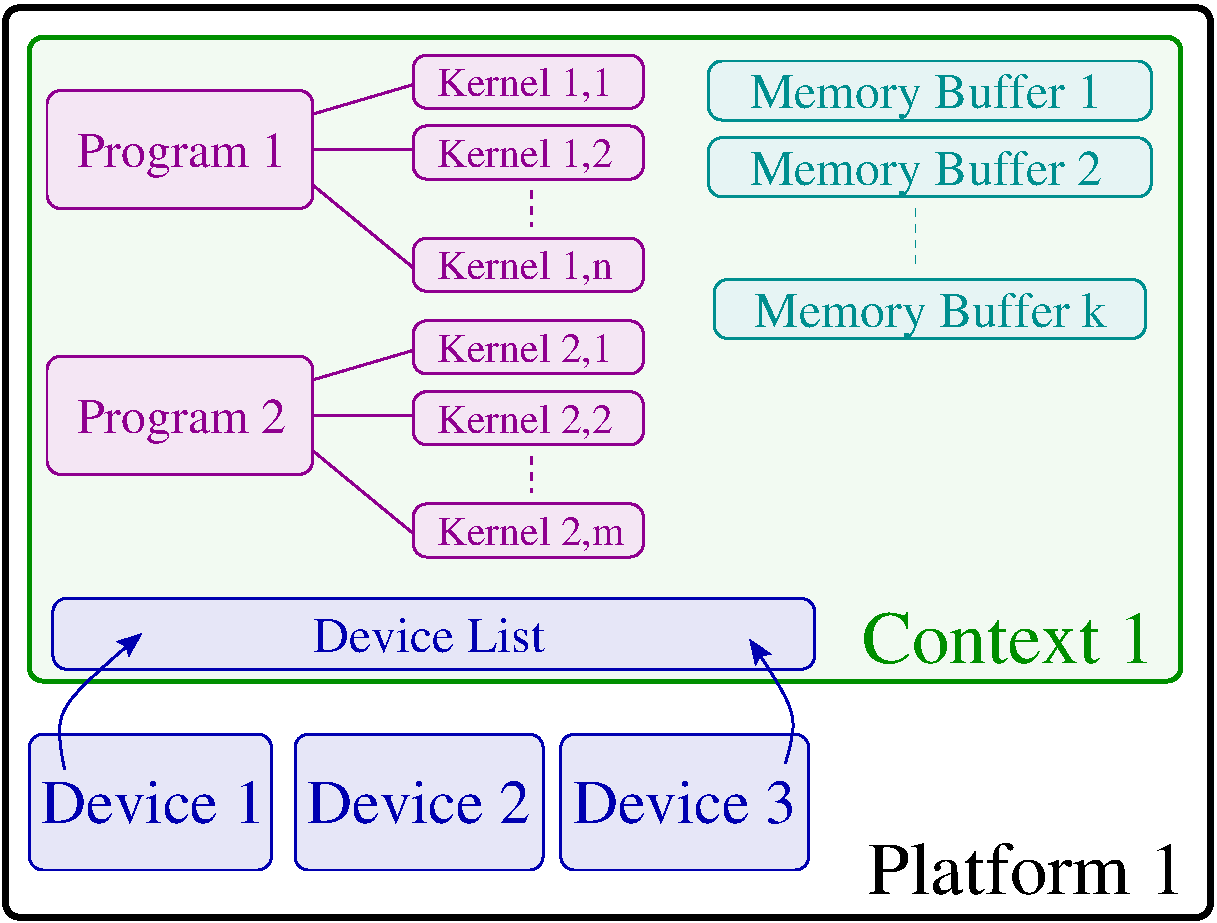
\includegraphics[width=0.85\textwidth]{figs/opencl-8.pdf}
 \end{center}
\end{frame}

\begin{frame}{OpenCL Platform Model}
 \begin{center}
   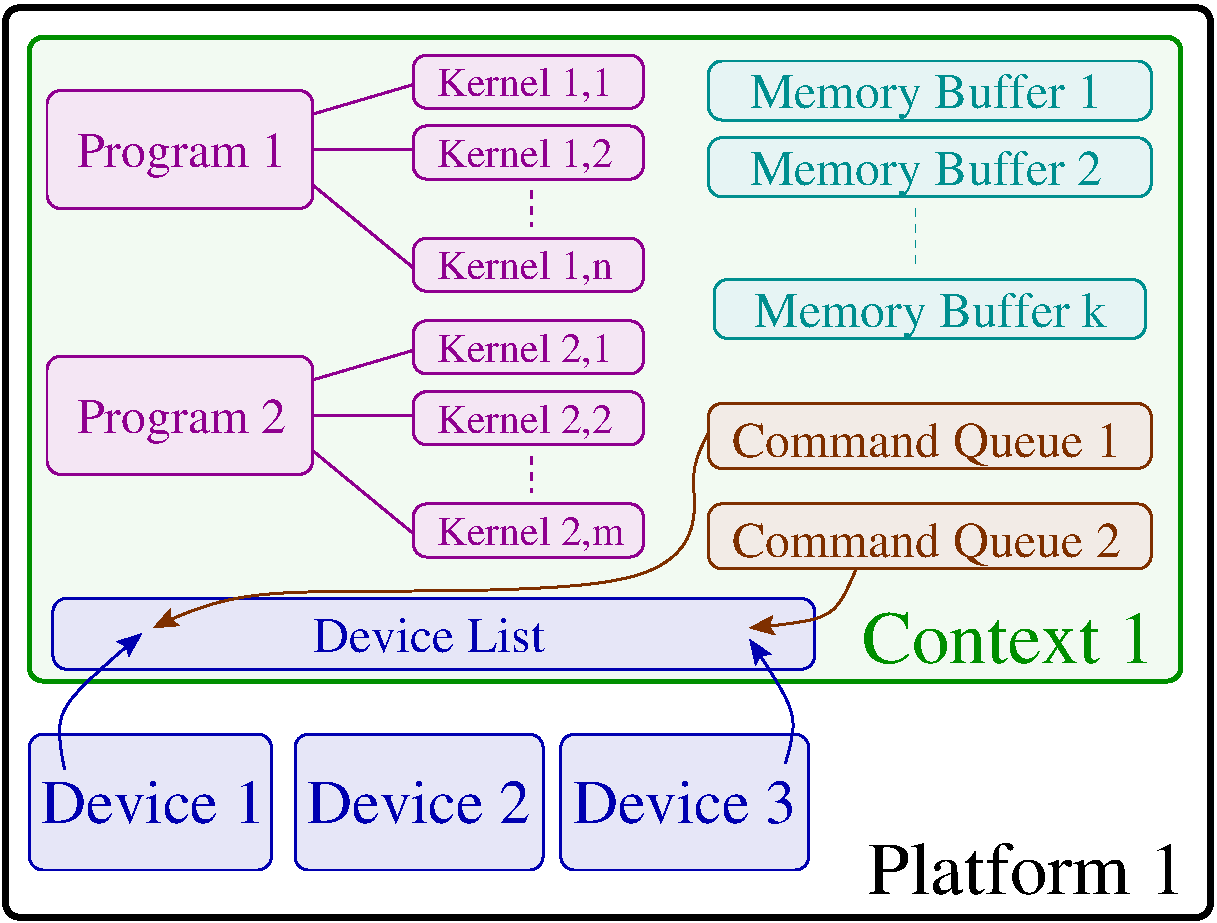
\includegraphics[width=0.85\textwidth]{figs/opencl-full.pdf}
 \end{center}
\end{frame}


%%%%%%%%%%%%%%%%%%%% Platform Model %%%%%%%%%%%%%%%%%%%%%%


\begin{frame}[fragile]
\frametitle{OpenCL Host API}

\lstset{ basicstyle=\scriptsize\ttfamily }
\begin{lstlisting}[escapechar=@]
@\color{red}{context}@ = clCreateContextFromType(NULL, CL_DEVICE_TYPE_GPU, NULL, NULL, NULL);
@\color{red}{queue}@ = clCreateCommandQueue(context, NULL, 0, NULL);
@\color{red}{memobjs[0]}@ = clCreateBuffer(context, CL_MEM_READ_WRITE, sizeof(float)*2*num_entries, NULL, NULL);
@\color{red}{memobjs[1]}@ = clCreateBuffer(context, CL_MEM_READ_ONLY | CL_MEM_COPY_HOST_PTR, sizeof(float)*2*num_entries, srcA, NULL);
 
@\color{red}{program}@ = clCreateProgramWithSource(context, 1, &kernel_src, NULL, NULL);
clBuildProgram(program, 0, NULL, NULL, NULL, NULL);
 
@\color{red}{kernel}@ = clCreateKernel(program, "my_kernel", NULL);
clSetKernelArg(kernel, 0, sizeof(cl_mem), (void *)&memobjs[0]);
clSetKernelArg(kernel, 1, sizeof(cl_mem), (void *)&memobjs[1]);
clSetKernelArg(kernel, 2, sizeof(float)*(local_work_size[0]+1)*16, NULL);
 
global_work_size[0] = 128;
 local_work_size[0] = 64;
clEnqueueNDRangeKernel(queue, kernel, 1, NULL, global_work_size, local_work_size, 0, NULL, NULL);
\end{lstlisting}
\lstset{ basicstyle=\small\ttfamily }

\begin{block}{Issues}
 \begin{itemize}
  \item ``Where is the error?''
  \item Manage OpenCL handles
 \end{itemize}

\end{block}

\end{frame}


\begin{frame}[fragile]
\frametitle{OpenCL Kernel Language}

\begin{block}{Sample Operation: Inplace Vector Addition}
 \vspace*{-0.5cm}
 \begin{align*}
  \left(
  \begin{array}{c}
   v_1^1 \\
   v_1^2 \\
   \vdots \\
   v_1^n 
  \end{array} \right) +\!= 
  \left(
  \begin{array}{c}
   v_2^1 \\
   v_2^2 \\
   \vdots \\
   v_2^n 
  \end{array} \right)
 \end{align*}
\end{block}

 \vspace*{-0.3cm}
\begin{block}{OpenCL Kernel}
\begin{lstlisting}
__kernel void inplace_add(
          __global const float * vec1,
          __global const float * vec2,
          unsigned int size) 
{ 
  for (unsigned int i  = get_global_id(0); 
                    i  < size; 
                    i += get_global_size(0))
    vec1[i] += vec2[i];
}
\end{lstlisting}
\end{block}

\end{frame}


%%%%%%%%%%%%%%%%% OpenCL closing %%%%%%%%%%%%%%%
% \begin{frame}{OpenCL Management}
%  \begin{center}
%    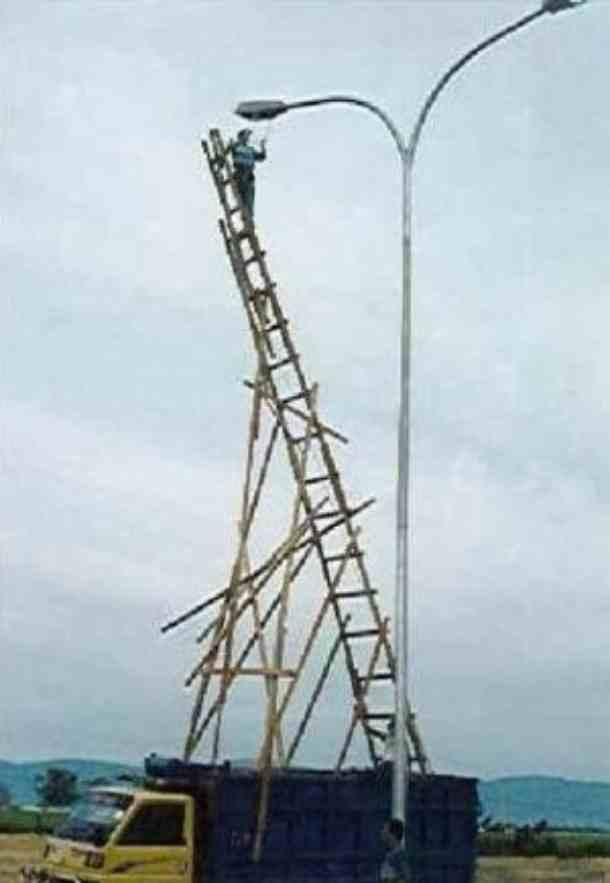
\includegraphics[width=0.45\textwidth]{figs/work1.jpg}
%  \end{center}
% \end{frame}


